\maketitle

\section{서론}

% 이미 AI 스피커를 중심으로 IoT를 구현하려는 시도는 보편적.
% 최근 LLM의 발전으로 이러한 AI 인터랙션이 더욱 많은 가능성을 내비치고 있음.
% LLM을 통해 다양한 기기를 조직하여 사용하면 어떨까?
% 어떤 기기가 작동 완료되면 이어서 다른 기기를 작동시키는 등 트리거 정의 가능.
% 특정 시간에 반복된 루틴을 설정할수도.

% 하지만 컴퓨터와 자연어로 소통하는 것은 쉬운 일이 아님.
% 특히 AI 스피커와 같은 홈 어시스턴트에게는 주어를 명확히 설명해야 하기 때문에 인터랙션의 병목.
% 자연어를 이해하는 홈 어시스턴트는 "이거", "저거"와 같은 지시대명사도 이해할 수 있어야.

% 특히 실내 공간이 한정적인 1인 가구에게 자연어를 이해하는 홈 어시스턴트는 매유 유용할 것.

오늘날 AI 스피커를 중심으로 IoT 환경을 구현하는 접근은 매우 일반적이다. 최근에는 LLM의 비약적인 발전으로 이러한 AI와의 음성 인터랙션이 더욱 많은 가능성을 보여주고 있다. 하지만 실제 용례를 살펴보면 AI와 자연어로 상호작용하는 방식이 매끄러운 사용자 경험을 제공하지는 못하고 있다. 특히 AI 스피커를 통해 제공되는 홈 어시스턴트에게는 사용자가 `어떤 대상을 어떻게 조작하고 싶은지' 명확히 설명해야 하는데, 이 과정에서 인터랙션의 병목이 발생한다.

이러한 문제의식을 배경으로, 나는 사용자의 제스처를 이해하는 홈 어시스턴트 인터랙션을 제안한다. 제스처를 이해하는 홈 어시스턴트는 기존과 같은 방식으로 사용자의 자연어 명령을 이해하는 것을 넘어서, 사용자가 대상을 손가락으로 가리키면서 ``이거", ``저거"와 같은 지시대명사를 사용했을 때 그 의미를 이해할 수 있다. 또한 TV의 볼륨을 조절하거나 조명의 밝기를 조절하고 싶을 때는 손 동작을 통해 어느정도로 값을 변경하고 싶은지 표현할 수 있다. 이렇게 제스처와 음성이 결합된 인터랙션을 통해 사용자는 더욱 효과적으로 홈 어시스턴트를 사용할 수 있다.

이 글에서는 페르소나를 정의한 뒤, 과업 분석 기법 중 시나리오 분석법을 통해 현재 사용자가 겪는 문제를 묘사한다. 이어서 사용자가 제스처를 인식하는 홈 어시스턴트를 사용하는 시나리오를 기술하여 어떻게 문제를 해결할 수 있는지 제시하고, 기대효과를 논하며 마친다.

\section{페르소나 및 시나리오 분석}

\textbf{이태영(28, 남성), 프로그래머, ``홈 어시스턴트가 내 명령을 더 잘 이해하면 좋겠어"}

28세 남성 이태영은 성남시의 19평 원룸에 거주하는 프로그래머다. 일상의 모든 것을 자동화하는 습관을 가진 이태영은 홈 어시스턴트 기능을 탑재한 AI 스피커를 사용하고 있다. 이태영은 음성을 통해 어시스턴트에게 명령을 내리곤 한다. 어시스턴트는 현관문, 창문, 커텐 등 가구와 냉장고, TV 등 가전에 연결되어 있고, 이들을 통제할 수 있다. 이태영은 잠들기 전 홈 어시스턴트를 호출한 뒤 ``TV 꺼줘"라고 명령하여 TV를 끈다. 이어서 거실에 있는 두 개의 전등을 끄기 위해 ``거실 1번, 2번 전등 꺼줘"라고 명령한다. 하지만 실제로 이태영이 끄고자 의도한 전등은 거실 2번이 아닌 3번 전등이었다. 이태영은 끄고 싶은 전등의 식별 이름이 기억나지 않아 결국 스마트폰의 홈 어시스턴트 앱을 통해 거실 3번 전등을 끈뒤 잠에 든다.

다음 날 아침 8시, 홈 어시스턴트는 예약된 루틴에 따라 커텐을 열고 아침 뉴스를 브리핑 해준다. 잠에서 덜 깬 이태영이 홈 어시스턴트의 소리를 줄이기 위해 어시스턴트를 호출한 뒤 ``볼륨 줄여줘"라고 말한다. 그러자 어시스턴트는 설정된 값만큼의 볼륨을 줄인다. 하지만 볼륨이 너무 작아서 뉴스가 들리지 않자 이태영은 ``볼륨 조금만 키워줘"라고 말한다. 명령대로 어시스턴트는 볼륨을 키웠지만, 그러자 처음 볼륨으로 돌아가서 소리가 너무 커지고 말았다. 짜증이 난 이태영은 자리에서 일어나 스마트폰의 홈 어시스턴트 앱으로 직접 볼륨을 `42'에 맞춘다.

첫 독립을 맞아 자신만의 스마트 홈을 구축하고 싶었던 이태영은 홈 어시스턴트에 많은 기대를 했지만, 실제로는 AI 스피커와 상호작용하는 것이 매우 번거롭고, 홈 어시스턴트에 연동된 다양한 기기를 음성만으로 조작하는 것이 쉽지 않다고 생각하고 있다.

\section{사용 시나리오}

% 자기 전 책을 읽으려고 누움. 램프는 켜고 전등을 끄고 싶을 때, 손가락으로 전등을 가리키며 꺼달라고 하면 꺼주고, 램프를 가리키며 켜달라고 하면 켜줌. 일련의 동작을 학습시켜서 "잘 준비해줘" 할 수도.

% "내일 아침 11시에 커텐 올려줘", "어떤 커텐 말씀이신가요?", "이거"

% <사진>

\vspace{-1mm}
\begin{figure}[h]
  \centering
  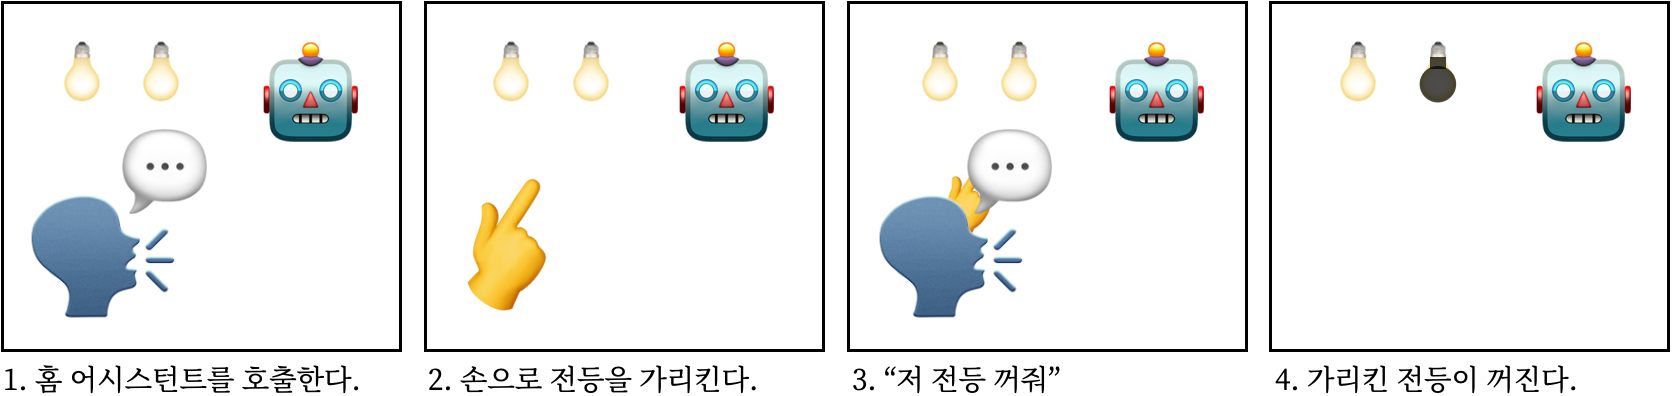
\includegraphics[width=\columnwidth]{sc1.png}
  \caption{지시 제스처를 이용한 명령 대상 선택 시나리오.}
  \label{fig:sc1}
\end{figure}
\vspace{-5mm}
\begin{figure}[h]
  \centering
  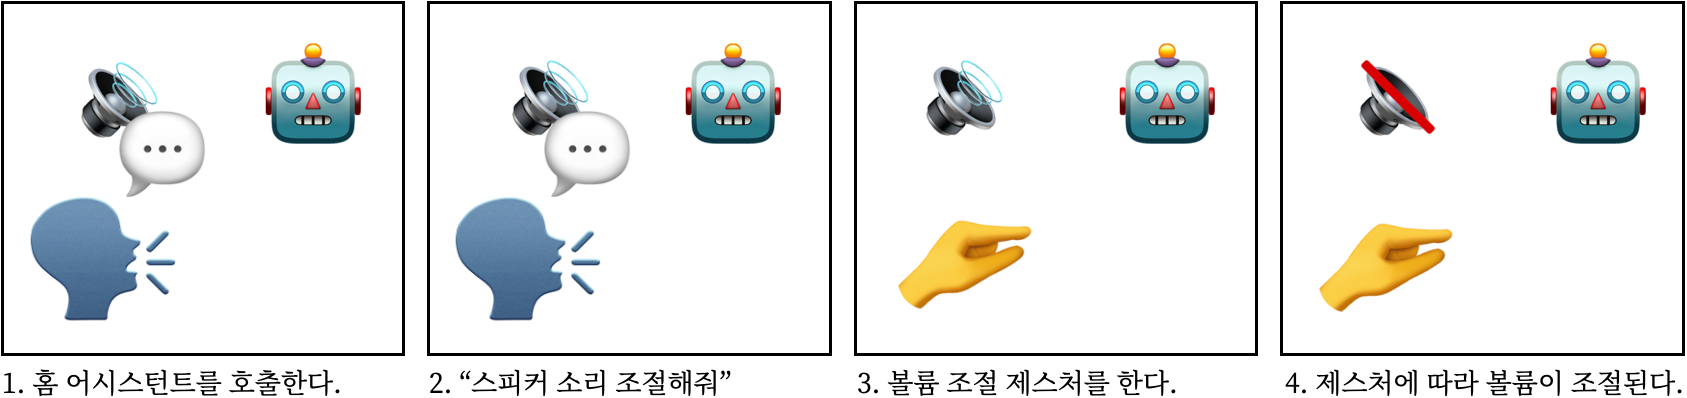
\includegraphics[width=\columnwidth]{sc2.png}
  \caption{제스처를 이용한 명령 수행 시나리오.}
  \label{fig:sc2}
\end{figure}
\vspace{-4mm}

이제 이태영은 제스처를 이해하는 홈 어시스턴트를 사용한다. 이태영은 전등을 끄고 싶을 때 \cnm{그림 \ref{fig:sc1}}과 같이 손가락으로 끄고 싶은 전등을 가리키며 ``저 전등 꺼줘"라고 말한다. 홈 어시스턴트는 이태영이 가리키는 전등을 확인하고 해당 전등을 꺼준다. 또한 스피커의 소리를 줄이고 싶을 때도 단순히 볼륨을 줄여달라고 명령하거나 볼륨의 크기 값을 직접 말하는 대신 \cnm{그림 \ref{fig:sc2}}와 같이 ``스피커 소리 조절해줘"라고 말한 뒤, 제스처를 이용해 볼륨을 어떻게 변경할지 표현할 수 있다. 이태영이 볼륨을 조절하기 위해 두 손가락을 들면 어시스턴트는 이 초기 손가락 거리를 기반으로 두 손가락의 거리가 멀어지면 볼륨을 높이고, 손가락의 거리가 짧아지면 볼륨을 줄여준다. 이태영은 자신의 손 동작에 따라 소리의 크기가 달라지는 것을 들으며 적절한 볼륨을 찾고, ``이 볼륨으로 설정해줘"라고 말해 상태를 확정한다. 기존에는 사용자의 명령과 어시스턴트의 응답이 일정한 간격을 두고 순차적으로 이뤄졌다면, 이제는 손가락을 움직일 때마다 실시간으로 피드백을 받는 인터랙션이 가능해진 것이다.

\section{기대효과 및 결론}

제스처를 이해하는 홈 어시스턴트는 음성만으로 제어해야 했던 기존 홈 어시스턴트에 비해 사용자 명령의 입체적인 맥락을 이해할 수 있다. 실제로 사람과 사람의 대화에서도 제스처와 같은 비언어적 표현이 큰 영향을 미치는 만큼, 인간과 AI 사이에서도 기존과 다른 수준의 인터랙션이 가능해질 것이다. 또한 제스처를 이해하는 홈 어시스턴트는 단순히 기존 사용자군의 사용성을 제고하는 것을 넘어서, 홈 어시스턴트가 수어를 인식할 수 있도록 만듦으로써 청각장애인과 같이 AI 스피커 사용에 제약이 있던 사용자들에게도 큰 도움이 될 수 있다.

기술적 구현은 이 글의 범위를 넘어서는 것이지만, LLM과 LiDAR를 결합하는 방식으로 프로토타입을 제작할 수 있을 것이며, 이렇게 구현된 홈 어시스턴트는 원룸과 같이 제한적인 공간에서 가장 이상적으로 동작할 수 있을 것이다. 또한 웨이크 업(Wake-up) 단어를 언급했을 때만 제스처를 추적하고, 클라이언트에서 분석까지 마친 뒤 서버에는 완결된 프롬프트만을 전송하도록하면 프라이버시 이슈를 피하는 것이 가능하다. 이처럼 제스처를 이해하는 홈 어시스턴트는 기존 문제를 해결하면서 유용성과 사용성을 갖춘 동시에, 실현 가능성도 충분한 제안이라고 할 수 있다.
